\documentclass[12pt]{article}
\special{papersize=3in,5in}

%-------------------------------------------------------
% PACKAGES

\usepackage[utf8]{inputenc}
\usepackage{amssymb,amsmath}
\usepackage{natbib}
\usepackage{outlines}
\usepackage{pgfgantt}
\usepackage{pdflscape}
\pagestyle{empty}
\setlength{\parindent}{0in}

\usepackage{bibentry}
\nobibliography*

%-------------------------------------------------------
% CONFIG

\author{Francisco Alves}
\title{Assessing Default Probabilities in Subnational Governments: The Case of Brazil}
\date{Dissertation Proposal (kind of)}

%-------------------------------------------------------
% BODY

\begin{document}

\maketitle

%-----------------------------------------------

\section{Introduction}

There is a clear consensus both in the academic literature and in the policy debate that sound management of fiscal risks is essential for both fiscal sustainability and macroeconomic stability of sovereign countries \citep{brixi2002, kopits2014, imf2016}. One of the classes of fiscal risks that were particularly neglected in the usual fiscal sustainability analysis is that related to contingent liabilities, that is, liabilities whose occurrences depends on the outcome of an uncertain event \citep{brixi2002}. A second important development in recent years is that with the increased decentralization in the provision of public services, the contingent liabilities, both explicit and implicit, arising from subnational governments (SNGs) are increasingly relevant for fiscal sustainability analysis. This relevance is higher the more spending and taxation powers are given to the subnational entities in the fiscal framework currently in place in a given country.

Although the above characterization could be employed to describe the recent economic history of several countries, Brazil might as well be the canonical example. A federation with one Federal District, 26 states, and 5,570 municipalities, Brazil experienced in the 80s and 90s repeated fiscal crisis of subnational entities with three rounds of debt restructurings. These episodes severely threatened the success of several macroeconomic stabilization programs that hoped to control the three-to-four-digit annual inflation rates that wreak havoc the Brazilian economy from 1980 through 1994. It was only with the success of the Real Plan in fighting the hyperinflation, and with a more comprehensive debt restructuring that aimed to correct the underlying SNG fiscal problems, that the political and economic conditions enabled for a complete reformulation of the fiscal institutions in place culminating with the publication of a Fiscal Responsibility Law (FRL) in 2000 \citep[p. 34-35]{manoel2013}. 

The FRL was a comprehensive law that promoted several changes in the institutions related to the Brazilian budgetary process. However, for the purposes of this study, the focus will be on the controls that were put forth for SGNs borrowings. Following the typology of borrowing controls used by \citet{ahmad2005} and first proposed by \citet{ter1997}, Brazil has adopted both a rules-based control and an administrative control for SNG borrowing. In a rules-based control, a fiscal rule is imposed that directly constrains the SNG ability to borrow. In Brazil, the FRL adopted both a golden rule and a debt ceiling rule. In an administrative control, the central government has some form of direct control over the SGN borrowing. In Brazil, if the central government must offer a guarantee for an individual borrowing operation, then the Finance Ministry, through the National Treasury Secretariat (STN), must assess that entity ``payment capacity'' before the operation is authorized.

The current methodology employed by STN was enacted in 2012 and makes use of several fiscal indicators to classify the SGNs entities in different credit classifications, similar in spirit to the process adopted by rating agencies in giving credit ratings. However, this methodology is currently being revised \footnote{The STN published the new set fiscal indicators and opened the methodology for a public revision process in the period of 10/05/2017 to 30/06/2017 at the website \url{http://www.tesouro.fazenda.gov.br/sistemagarantiauniao}}, as the STN is looking for an alternative suite of fiscal indicators that are more transparent and more easily calculated. In this context, the assessement of the statistical and economic significance of both the current and the newly set of fiscal indicators used by the National Treasury Secretariat to assess the solvency of subnational governments in Brazil in borrowing operations where the federal government needs to provide debt guarantees for the creditors is both necessary and timely.

The strand of literature on Early Warning Systems for economic crisis are particularly relevant for this endeavour. Following the seminal work by \citet{kaminsky1998} and \citet{berg1999} on currency crisis, it was not long until fiscal crisis were also tackled \citep{manasse2003, baldacci2011b, berti2012, dawood2017}. In this study, the focus will be on what is usually called the parametric approach, that makes use of limited dependent variables models, such as probit and logit. There are three main contributions. First, as usually true in most countries, disaggregate fiscal data on regional governments tends to have a much lower quality and standardization then on central governments for the obvious reasons\footnote{Although there are several initiatives in place in Brazil to modernize the information available for SNGs, in the fiscal transparency evaluation conducted by the IMF in Brazil completed in June 2016 and published in May 2017 it is noted that ``Weaknesses in fiscal reporting also undermine the ability to assess the fiscal position and risks. Not all states and municipalities comply with their reporting obligations, and information on subnational finances is generally less timely and comprehensive than information on the central governments. \citep[p. 62]{imf2017}''}. This study aims to compile, consolidate and make available on machine readable format regional discriminated data on the fiscal variables for the states that can be used to produce statistics comparable to those put forth on the 2014 Government Finance Statistical Manual \citep{imf2014}. To the best of the author's knowledge, this type of information is virtually inexistent today. The second contribution is the application of the Early Warning System literature on subnational governments. Most of the studies focus on sovereign governments, but, as noted by \citet{ianchovichina2007}, SGNs are sufficiently different from sovereign governments and demand separate analysis. The third and final contribution is that by recognizing a fiscal crisis as a rare event as suggested by \citet{king2001a}, that is, a binary dependent variable with dozens to thousands of times fewer ones than zeros, we make use of the correction proposed by \citet{king2001b} in order to correct for the bias that tends to sharply underestimate the probability of rare events.

\newpage
\section{Literature Review}

\textbf{On fiscal sustainability}

\begin{itemize}
\item \bibentry{burnside2005}
\item \bibentry{ianchovichina2007}
\end{itemize}

\textbf{On fiscal risks}

\begin{itemize}
\item \bibentry{brixi2002}
\item \bibentry{kopits2014}
\item \bibentry{bachmair2016}
\item \bibentry{imf2016}
\end{itemize}

\textbf{On subnational governments}

\begin{itemize}
\item \bibentry{ahmad2005}
\item \bibentry{liu2010}
\item \bibentry{canuto2013}
\end{itemize}

\textbf{On fiscal crisis in Brazil}

\begin{itemize}
\item \bibentry{manoel2013}
\end{itemize}

\textbf{On fiscal indicators and fiscal variables}

\begin{itemize}
\item \bibentry{baldacci2011a}
\item \bibentry{imf2014}
\item \bibentry{imf2015}
\end{itemize}

\textbf{On early warning systems (EWS) for currency and financial crisis}

\begin{itemize}
\item \bibentry{kaminsky1998}
\item \bibentry{berg1999}
\item \bibentry{berg2005}
\item \bibentry{candelon2012}
\item \bibentry{comelli2014}
\end{itemize}

\textbf{On early warning systems (EWS) for fiscal crisis}

\begin{itemize}
\item \bibentry{manasse2003}
\item \bibentry{baldacci2011b}
\item \bibentry{berti2012}
\item \bibentry{dawood2017}
\end{itemize}

\textbf{On logit estimates in rare events data}

\begin{itemize}
\item \bibentry{king2001a}	
\item \bibentry{king2001b}
\end{itemize}

The following also constitute valuable references that will be consulted as nedeed

\begin{itemize}
\item Relevant standards and codes recommendations (ex: Fiscal Transparency Code, PEFA, DeMPA, etc)
\item Rating criteria and methodology (ex: Moody's, Standard \& Poor's and Fitch Ratings)
\item Fiscal Councils publications (ex: Irish Fiscal Advisory Council, Office for Budget Responsibility, Council for Budget Responsibility, etc)
\item Relevant brazilian legislation (ex: Fiscal Responsibility Law, 2016 Debt Relief Plan for the States and the Federal District Law, National Treasury Secretariat Payment Capacity Evaluation Methodology, etc)
\item Econometric and Statistical Textbooks 
\end{itemize}

\newpage
\section{Methods}

\subsection{Data}

The majority of the explanatory variables used in this study will be fiscal variables and indicators derived from the datasets provided by the National Treasury Secretariat (STN). This section aim is to address the main data gaps that prevent the use of some specific years in the empirical analysis of this study. The original period covered by the data published by STN extends through 1986 through 2016, totalling 31 years of data. 

The first issue arises in the period from 1980 through 1994 when Brazil was facing a hyperinflation crisis and used several different currencies. Taking into considerations the difficulty in compiling accurate statistics during a period in which prices are changing so rapidly, the possible relevant period is shortened to 1995-2016. 

The second issue is related to the change in fiscal reporting practices brought about by the the Fiscal Responsibility Law in 2000-05-04 and the change in the Economic Classification of expenditures in 2001-05-04. Before this period, only flow variables are published by the STN, and they are not fully consistent with the more recent series. Taking into account the relevance of stock variables for fiscal analysis, the period is again shortened to 2002-2016.

The final issue is related to the conditions surrounding the bailouts provided by the National government. The states were allowed a cap on the maximum amount of debt service that they needed to pay in any given year in terms of their net revenue (Receita Liquida Real), with the difference being incorporated into the debt stock. However, instead of using an accrual basis of accounting, only the interest paid was registered. The central back publishes statistics on an accrual basis for regional governments, but they only begin in 2008. Taking into consideration the relevance of this variable, the period is again shortened to 2008-2016.

\subsubsection{Ethical Considerations}

All the data used in this study are public available on the internet on the websites of the relevant public entities of the Brazilian Government, such as the National Treasury Secretariat and the Central Bank. Therefore, the author's role was related to data integration and cleansing.

\newpage
\section{Dissertation Plan}

\subsection{Dissertation Outline}

\begin{outline}
\1[I)] Introduction
\1[II)] Literature Review
    \2 Fiscal Sustainability (?)
    \2 Fiscal Risks
        \3 Frameworks (aka Management)
        \3 Tools (aka Measurement)
    \2 Early Warning Systems
        \3 Non-parametric
        \3 Parametric
    \2 Brazil Fiscal Framework
        \3 Brazil Subnational Debt Restructuring of the 1990s
        \3 Fiscal Responsibility Law
        \3 2016 Debt Relief Plan for the States and the Federal District (PLP 257/2016, LC 156/2016)
        \3 Payment Capacity Evaluation Methodology
\1[III)] Methods
    \2[III.1)] Data
        \3 Data Source
        \3 Definitions of Explanatory Variables (Appendix?)
        \3 Descriptive Statistics
    \2[III.2)] Econometric Model
        \3 Limited Dependent Variable
        \3 Logit Regression
        \3 Rare Events
\1[IV)] Results
\1[V)] Conclusion
\end{outline}

\begin{landscape}

\subsection{Schedule}

\scalebox{0.6}{
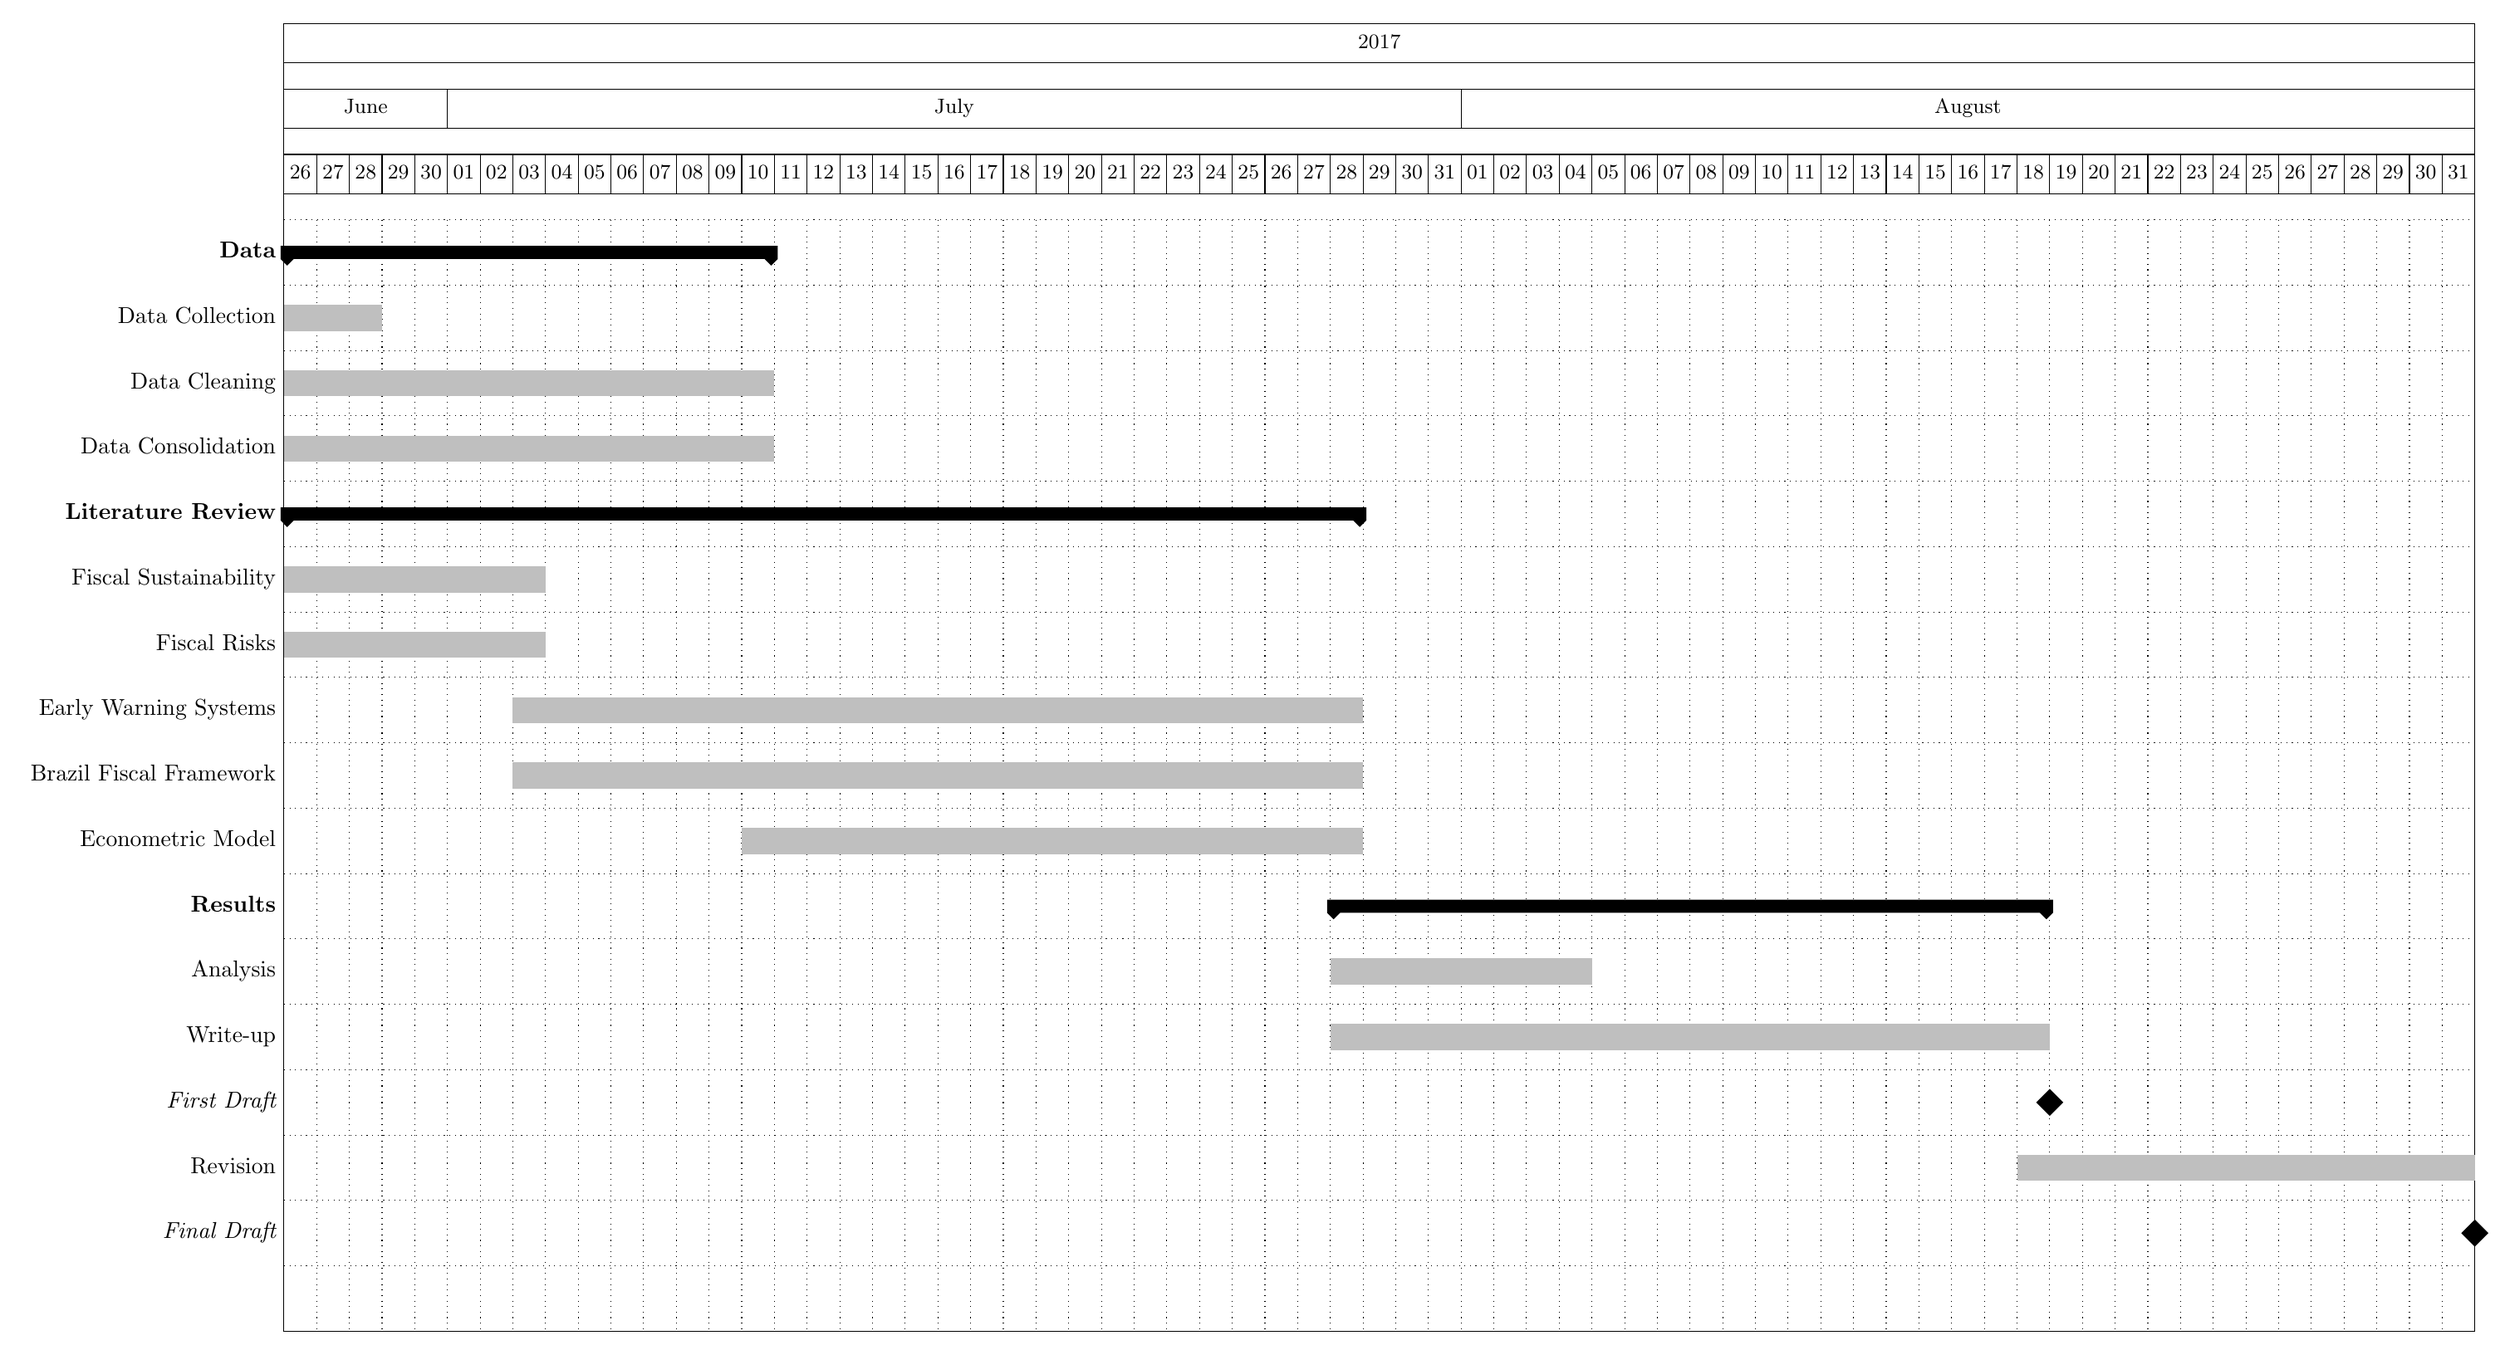
\begin{tikzpicture}
\begin{ganttchart}[
hgrid,
vgrid,
bar/.style={fill=gray!50},
time slot format=isodate
]{2017-06-26}{2017-08-31}

\gantttitlecalendar{year, month=name, day} \\

\ganttgroup{Data}{2017-06-26}{2017-07-10} \\
    \ganttbar{Data Collection}{2017-06-26}{2017-06-28} \\
    \ganttbar{Data Cleaning}{2017-06-26}{2017-07-10} \\
    \ganttbar{Data Consolidation}{2017-06-26}{2017-07-10} \\

\ganttgroup{Literature Review}{2017-06-26}{2017-07-28} \\
    \ganttbar{Fiscal Sustainability}{2017-06-26}{2017-07-03} \\
    \ganttbar{Fiscal Risks}{2017-06-26}{2017-07-03} \\
    \ganttbar{Early Warning Systems}{2017-07-03}{2017-07-28} \\
    \ganttbar{Brazil Fiscal Framework}{2017-07-03}{2017-07-28} \\

\ganttbar{Econometric Model}{2017-07-10}{2017-07-28} \\

\ganttgroup{Results}{2017-07-28}{2017-08-18} \\
    \ganttbar{Analysis}{2017-07-28}{2017-08-04} \\
    \ganttbar{Write-up}{2017-07-28}{2017-08-18} \\

\ganttmilestone{First Draft}{2017-08-18} \\

\ganttbar{Revision}{2017-08-18}{2017-08-31} \\

\ganttmilestone{Final Draft}{2017-08-31} \\


\end{ganttchart}
\end{tikzpicture}
} 

\end{landscape}

%-------------------------------------------------------
% REFERENCES
\bibliographystyle{apalike}
{\footnotesize
\bibliography{../../references.bib}}

\end{document}

